\begin{figure*}[t]
% \vspace*{-3mm}
\centerline{
\begin{tabular}{cccc}
    \hspace*{-2mm}  \includegraphics[width=0.25\textwidth,height=!]{figs/ua.pdf} &
    \hspace*{-5mm} \includegraphics[width=0.25\textwidth,height=!]{figs/mia.pdf} &
    \hspace*{-5mm} 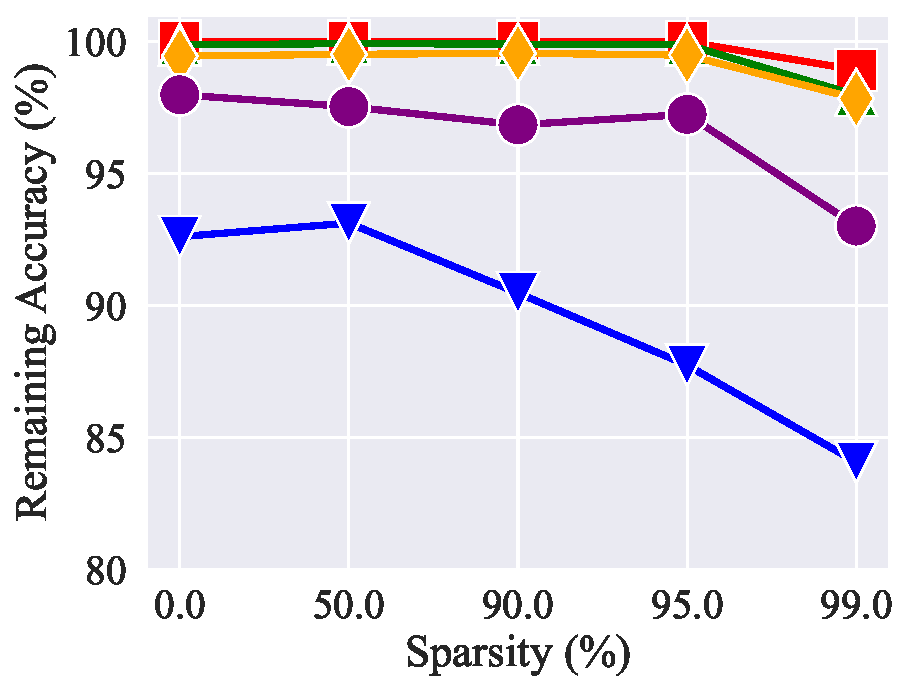
\includegraphics[width=0.25\textwidth,height=!]{figs/ra.pdf} &
    \hspace*{-5mm}  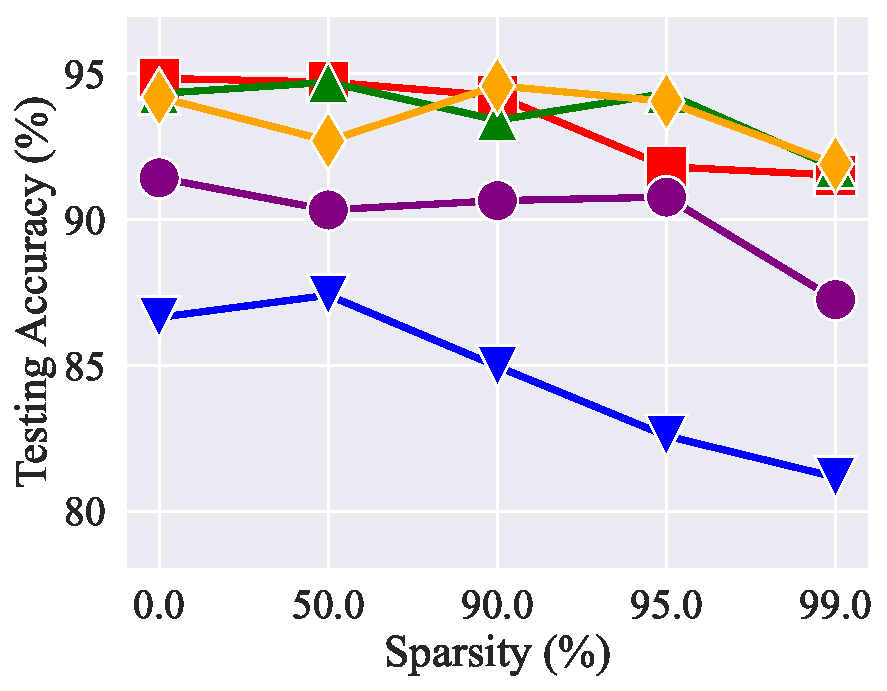
\includegraphics[width=0.25\textwidth,height=!]{figs/ta.pdf} 
\end{tabular}}
 \vspace*{-3mm}
\caption{\footnotesize{
%\SL{[Figure needs updating.]} %\JC{"Retain" -> "Remain"}
Performance of approximate unlearning ({\FTC}, {\GAC}, {\FFC}, {\IUC}) and exact unlearning ({\retrainC}) in efficacy ({\UA} and {\MIAF}), fidelity ({\RA}), and generalization ({\TA}) vs. model sparsity (achieved by {OMP}) in the data-model setup (CIFAR-10, ResNet-18). 
The unlearning scenario is class-wise 
 forgetting, and 
the average unlearning  performance over 10 classes is reported. We remark that being closer to \textcolor{red}{Retrain} performance is better for approximate MU schemes.
% \JC{TODO: Remove legend in fig 3c}
%\PS{See comment in the last para of Section 3. Are we trying to forget an entire class?}
}}
\vspace*{-7mm}
\label{fig: results_OMP_MU}
\end{figure*}